\documentclass[crop]{standalone}

\usepackage[usenames,dvipsnames]{xcolor}
\usepackage{tikz}

\definecolor{NODE}{HTML}{006400} % green

\usetikzlibrary{arrows,positioning}
\tikzset{
  treenode/.style = {
    align=center, 
    inner sep=0pt, 
    text centered,
    font=\sffamily,
    text width=1.5em,
    very thick,
    minimum width=1.5em, 
    minimum height=1.5em
  },
  N/.style = {
    treenode,
    circle,
    white,
    draw=black,
    fill=NODE,
    thin,
  },
  E/.style = {
    treenode,
    rectangle,
    white,
    draw=black,
    thin,
    scale=0.5
  },% arbre rouge noir, nil
  SUBTREE/.style = {
    treenode
  },
  level/.style = {
    sibling distance = 5cm/#1,
    level distance = 1.5cm
  }
}


\begin{document}

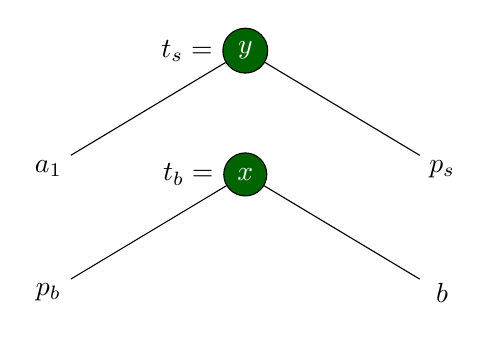
\begin{tikzpicture} 
  \node (fst) [N,label=180:{$t_s=$}] {$y$}
	child{ node [SUBTREE] {$a_1$} }
	child{ node [SUBTREE] {$p_s$} }
    ; 
  \node [below=of fst,N,label=180:{$t_b=$}] {$x$}
	child{ node [SUBTREE] {$p_b$} }
	child{ node [SUBTREE] {$b$} }
    ; 
\end{tikzpicture}

\end{document}
